\documentclass[12pt]{report}

%Vous souciez pas de tout les packages, j'ai oublié ce que fait la moitié d'entre eux

\usepackage[utf8]{inputenc}
\usepackage[T1]{fontenc}
\usepackage[francais]{babel}
%\usepackage{layout}
\usepackage[left=3cm,right=3cm,top=3cm,bottom=3cm]{geometry}
%\usepackage{setspace}
\usepackage{soul}
\usepackage[normalem]{ulem}
%\usepackage{eurosym}
%\usepackage{bookman}
%\usepackage{charter}
%\usepackage{newcent}
%\usepackage{lmodern}
%\usepackage{mathpazo}
%\usepackage{mathptmx}
%\usepackage{url}
%\usepackage{verbatim}
%\usepackage{moreverb}
%\usepackage{listings}
%\usepackage{fancyhdr}
%\usepackage{wrapfig}
\usepackage{color}
%\usepackage{colortbl}
\usepackage{amsmath}
\usepackage{amssymb}
\usepackage{mathrsfs}
%\usepackage{asmthm}
%\usepackage{makeidx}
\usepackage{graphicx}
\usepackage{tabularx}
\usepackage{tgtermes}
\usepackage{titlesec}
\usepackage[final]{pdfpages} 
\usepackage{epsfig}
\usepackage{comment}
\usepackage{float}
\usepackage{amsmath}
\renewcommand{\emph}{\textit}
\renewcommand{\thesection}{\arabic{section}}
\renewcommand{\thesubsection}{\arabic{section}.\arabic{subsection}}
\titleformat*{\subsection}{\bfseries}
\parskip=5pt

%Information pour la page de garde

\title{TP 3 - Le codage prédictif}
\author{Jean-Baptiste \bsc{Morice}, Guillaume \bsc{Versal}}
\date{\today}


\begin{document}



%Commande qui crée la page de garde
\maketitle

\tableofcontents

\newpage
\section*{Introduction}

Le but de ce TP était de nous faire réaliser un codeur basé sur du codage prédictif en boucle fermée. Pour mettre en place cette boucle nous avons aussi réalisé différents codeurs tels que le MIC Différentiel (monodirectionnel et bidirectionnel) et le MICD Adaptatif. Leurs implémentations nous étaient fournies dans le sujet de notre TP. De plus, nous devions évaluer la performance des différents prédicteurs et aussi mettre en place un système de quantification uniforme.


\newpage
\section{Notre travail}

\subsection{Étude de prédicteurs simples}

Dans un premier temps, notre travail a consisté en l'implémentation des différents codeurs cités plus haut (MICD mono, MICD bi et MICDA) puis en la réalisation d'une étude comparative des différents prédicteurs, grâce notamment à l'histogramme de l'erreur de prédiction ou au calcul du PSNR de l'image décodée avec l'image originale de référence.

\subsubsection{Choix des conditions aux bords}

Pour la prédiction mono-dimensionnelle,  nous prenons $P(X) = 128$ sur la première colonne. Pour les deux autres prédictions, on prendra aussi $P(X) = 128$ pour la première colonne et ligne. 

\emph{Ce choix était-il pertinent ?}

Le but de cette première prédiction est de minimiser l'erreur, c'est à dire de minimiser $E(i,j)$. Or, $E(i,j) = X(i,j) - X_p(i,j)$, il faut ainsi trouver la valeur de $X(i,j)$ qui minimise cette opération, et cette valeur c'est la moyenne de $X(i,j)$ c'est à dire 128.

\subsubsection{Performances des différents prédicteurs}

Dans ce TP, nous devions encoder l'image \texttt{boat.bmp} présente ci-dessous. Pour ce faire, nous avons seulement travaillé sur le canal Y de l'image comme sur les anciens TP. Cette image originale dispose d'une entropie de 6,69.

\begin{figure}[H]
\begin{center}
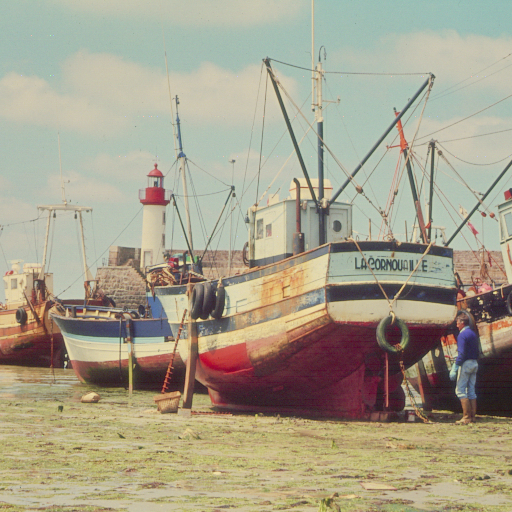
\includegraphics[scale=0.4]{../boats.jpg} 
\caption{Image originale en couleur}
\end{center}
\end{figure}

\begin{figure}[H]
\begin{center}
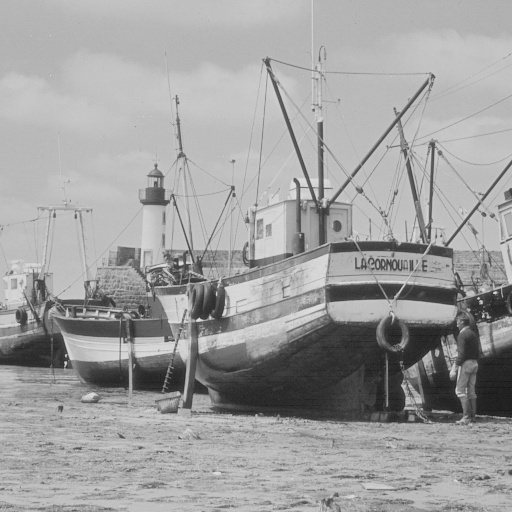
\includegraphics[scale=0.4]{../ImageRes/Imageoriginale.jpg} 
\caption{Image originale (uniquement le canal Y)}
\end{center}
\end{figure}

Dans un premier temps, nous avons appliqué les trois prédicteurs à l'image de base. Comme il n'y a pas de quantification, il n'y a pas de différence dans les images après qu'elles aient été décodée. Ainsi, on observe la différence entre les prédicteurs au niveau de l'erreur de prédiction transmise. 
Ce que l'on observe sur les images ci-dessous utilisant le MICD monodirectionnel, MICD bidirectionnel et MIDCA, c'est que l'erreur ressemble énormément à ce que l'on peut obtenir avec un gradient (ces images ont été normalisées pour les besoins du compte rendu). 

\begin{figure}[H]
\begin{center}
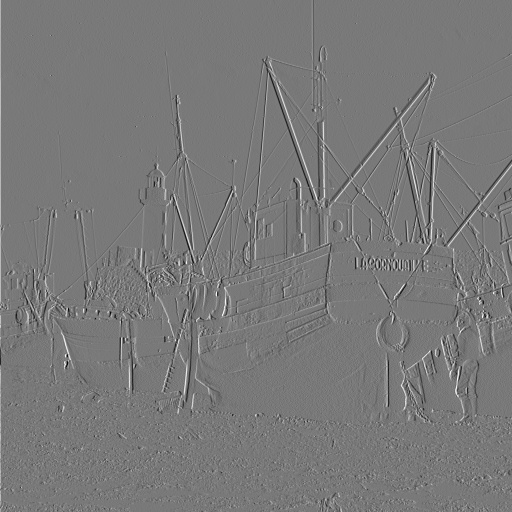
\includegraphics[scale=0.4]{../ImageRes/ImagecodeeMICDmonoQ1.jpg} 
\caption{Erreur avec la prédiction MICD mono}
\end{center}
\end{figure}

\begin{figure}[H][H]
\begin{center}
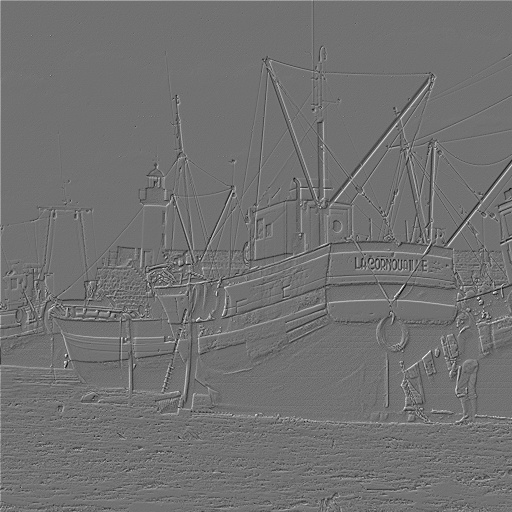
\includegraphics[scale=0.4]{../ImageRes/ImagecodeeMICDbiQ1.jpg} 
\caption{Erreur avec la prédiction MICD bi}
\end{center}
\end{figure}

\begin{figure}[H]
\begin{center}
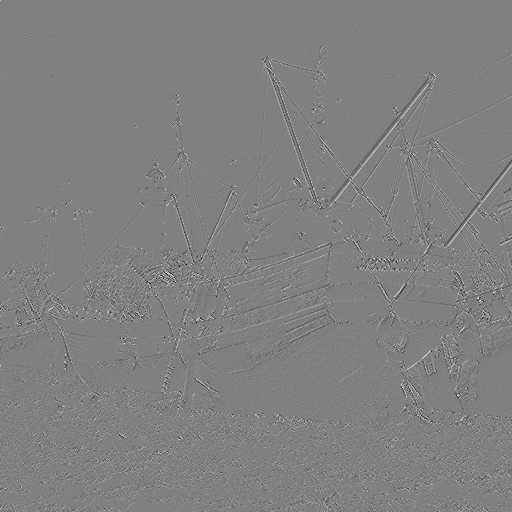
\includegraphics[scale=0.4]{../ImageRes/ImagecodeeMICDAQ1.jpg} 
\caption{Erreur avec la prédiction MICDA}
\end{center}
\end{figure}

Nous pouvons aussi constater sur les histogrammes que les différentes erreurs ont un histogramme plus ou moins semblable. Les différentes méthodes nous donnent aussi des entropies pour les images d'erreurs plus ou moins semblables allant de 4,8 pour le MICD monodirectionnel et le MIDCA, à 4,7 pour le MICD bidirectionnel qui semble un peu plus performant. Ce que l'on peut observer c'est que pour chacune de ces images d'erreur, l'entropie est largement plus faible que l'entropie de l'image originale. Ainsi, le codage prédictif et le schéma en boucle fermée montre bien son utilité sur une simple transmission de l'image.

\begin{figure}[H]
\begin{center}
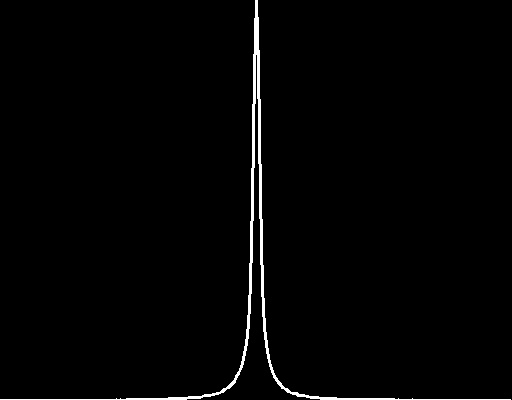
\includegraphics[scale=0.4]{../ImageRes/HistogrammeErreurMICDmonoQ1.jpg} 
\caption{Histogramme de l'erreur avec la prédiction MICD mono}
\end{center}
\end{figure}

\begin{figure}[H]
\begin{center}
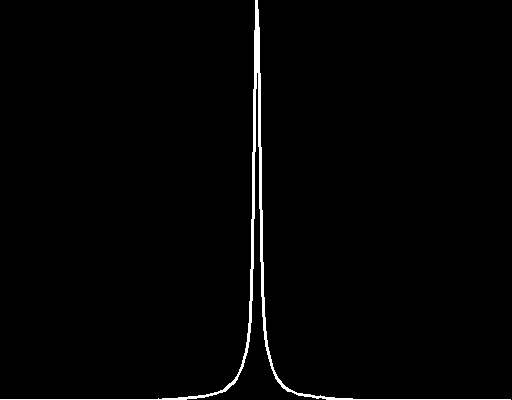
\includegraphics[scale=0.4]{../ImageRes/HistogrammeErreurMICDbiQ1.jpg} 
\caption{Histogramme de l'erreur avec la prédiction MICD bi}
\end{center}
\end{figure}

\begin{figure}[H]
\begin{center}
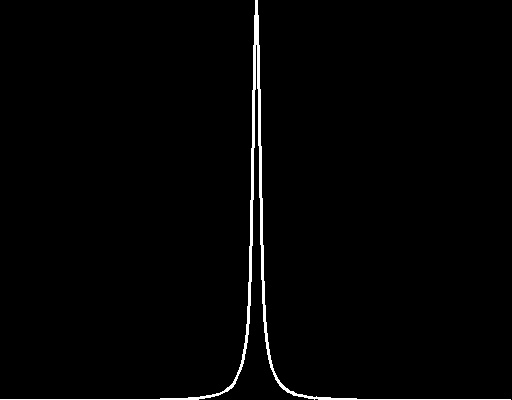
\includegraphics[scale=0.4]{../ImageRes/HistogrammeErreurMICDAQ1.jpg} 
\caption{Histogramme de l'erreur avec la prédiction MICDA}
\end{center}
\end{figure}

\subsubsection{Codage compétitif}

Ce que l'on peut observer sur les images d'erreur c'est que les prédicteurs ne réagissent pas de la même manière selon les endroits de l'image. Ainsi, il est intéressant d'utiliser le meilleur prédicteur pour un pixel donné dans le but de réduire l'entropie et c'est ce en quoi consiste le codage prédictif. Pour chaque pixel on teste le prédicteur qui minimisera l'erreur et ainsi l'information à transmettre.

Or, il est aussi nécessaire, avec cette façon de faire, de transmettre une seconde image qui informe le décodeur sur le prédicteur qui a été choisi. Cette carte des choix (présente ci-dessous) a une entropie proche de 1,3.

\begin{figure}[H]
\begin{center}
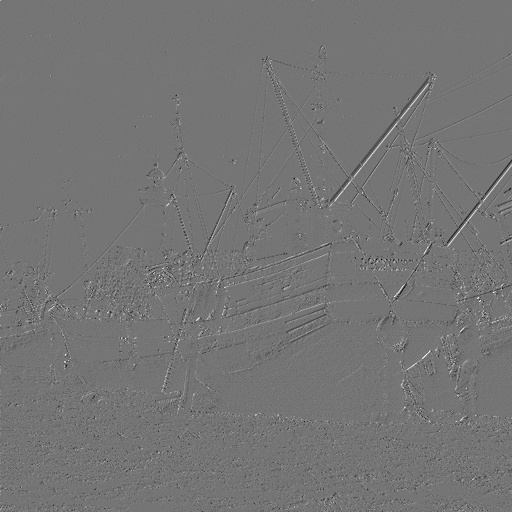
\includegraphics[scale=0.4]{../ImageRes/ImagecodeeCompetitifQ1.jpg} 
\caption{Erreur avec la prédiction compétitive}
\end{center}
\end{figure}

\begin{figure}[H]
\begin{center}
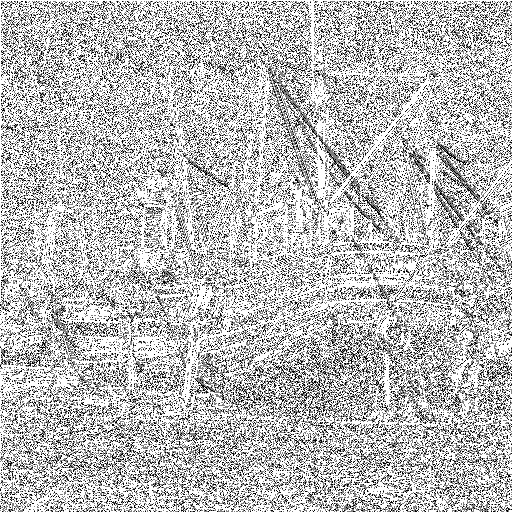
\includegraphics[scale=0.4]{../ImageRes/erreur.jpg} 
\caption{Erreur avec la prédiction compétitive}
\end{center}
\end{figure}

Concernant la carte d'erreur, on peut observer que l'entropie en compétitif est largement inférieure aux autres prédicteurs. Mais cela est à relativiser car il y à la transmission du choix.

\begin{figure}[H]
\begin{center}
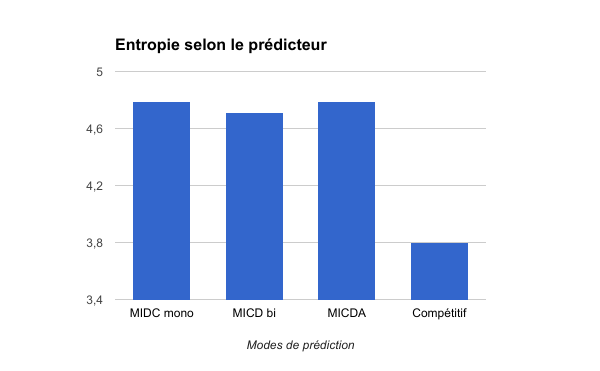
\includegraphics[scale=0.8]{../ImageRes/entropie.png} 
\caption{Comparaison des entropies}
\end{center}
\end{figure}

\subsection{Quantification uniforme}

Une autre méthode pour réduire l'entropie de l'information est de procéder à une quantification. Le souci de la quantification est que cette dernière produit une perte d'information qui ne sera pas retrouvée au décodage. Ainsi, l'image décodée se retrouvera altérée. Nous pouvons notamment l'observer sur le graphique ci dessous qui nous montre clairement la baisse de l'entropie lorsque le pas de quantification augmente.

\begin{figure}[H]
\begin{center}
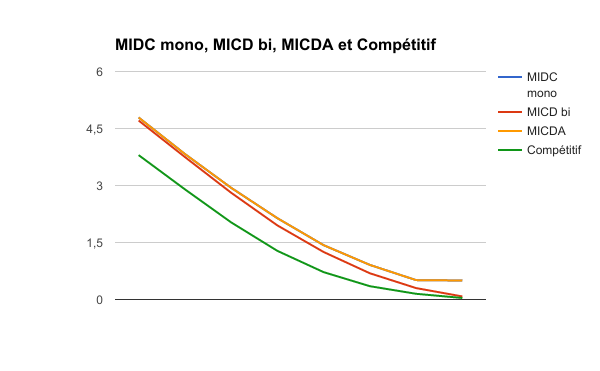
\includegraphics[scale=0.8]{../ImageRes/entropieQ.png} 
\caption{Entropie en fonction du pas de quantification}
\end{center}
\end{figure}

Malgré tout, même si la baisse de l'entropie est une bonne chose, cette dernière, comme dit précédemment, impacte le résultat final et donne une image de moins bonne qualité. Si la différence ne se fait pas sentir lorsque le pas de quantification est faible, lorsque ce dernier augmente trop cela produit des effets sur l'image. Les effets produits sont différents selon le prédicteur choisi : par exemple le MICD monodirectionnel et MICDA font tout deux rapidement disparaître les nuages dans le ciel, tandis que le MICD bidirectionnel laisse apparaître des traits diagonaux.

\begin{figure}[H]
\begin{center}
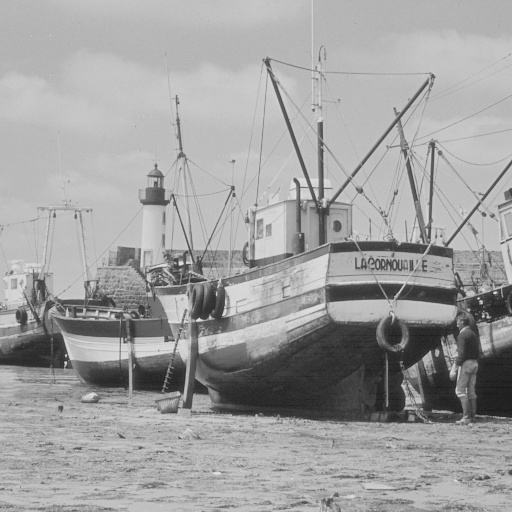
\includegraphics[scale=0.25]{../ImageRes/ImagedecodeeMICDmonoQ2.jpg} 
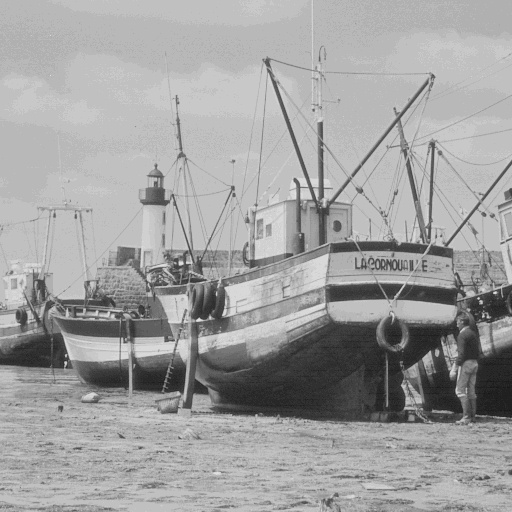
\includegraphics[scale=0.25]{../ImageRes/ImagedecodeeMICDmonoQ8.jpg} 
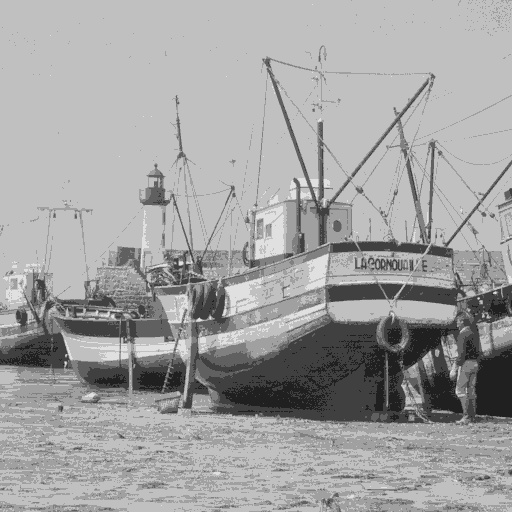
\includegraphics[scale=0.25]{../ImageRes/ImagedecodeeMICDmonoQ32.jpg} 
\caption{Images décodées en MICD mono avec un pas de 2,8 et 32 }
\end{center}
\end{figure}

\begin{figure}[H]
\begin{center}
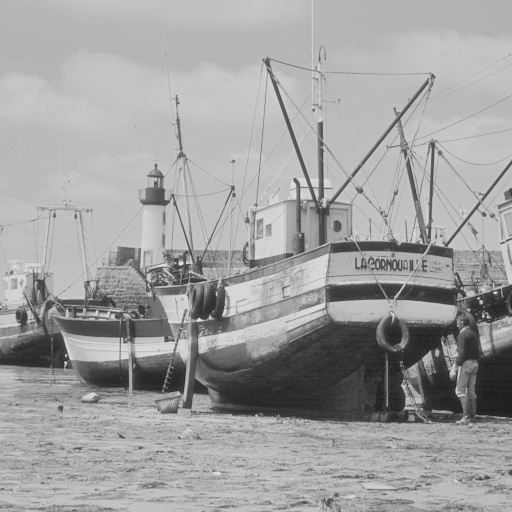
\includegraphics[scale=0.25]{../ImageRes/ImagedecodeeMICDbiQ2.jpg} 
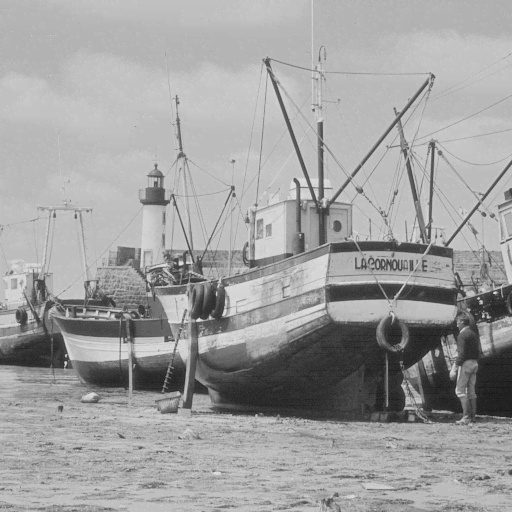
\includegraphics[scale=0.25]{../ImageRes/ImagedecodeeMICDbiQ8.jpg} 
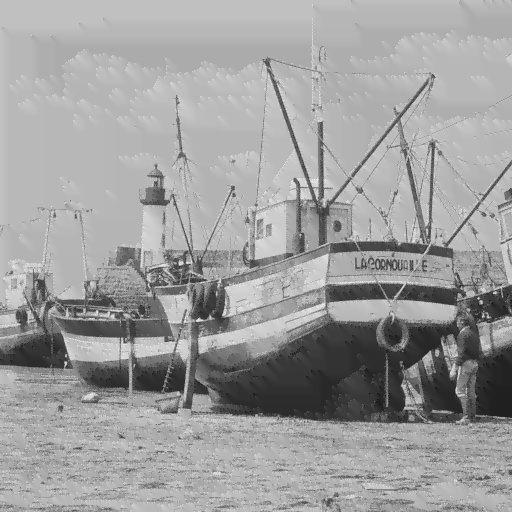
\includegraphics[scale=0.25]{../ImageRes/ImagedecodeeMICDbiQ32.jpg} 
\caption{Images décodées en MICD bi avec un pas de 2,8 et 32 }
\end{center}
\end{figure}

\begin{figure}[H]
\begin{center}
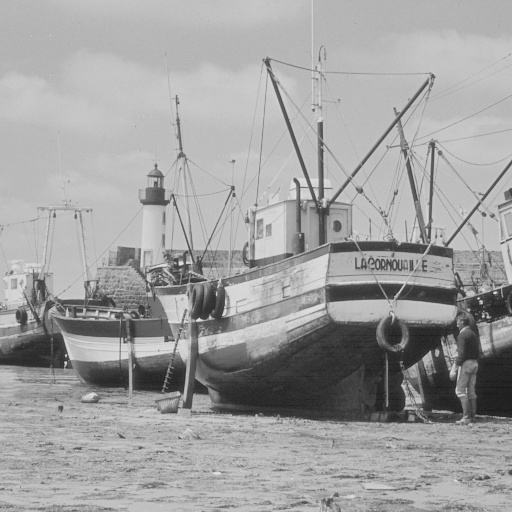
\includegraphics[scale=0.25]{../ImageRes/ImagedecodeeMICDAQ2.jpg} 
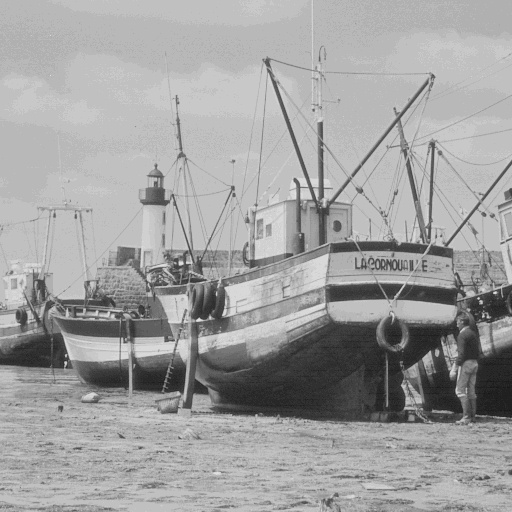
\includegraphics[scale=0.25]{../ImageRes/ImagedecodeeMICDAQ8.jpg} 
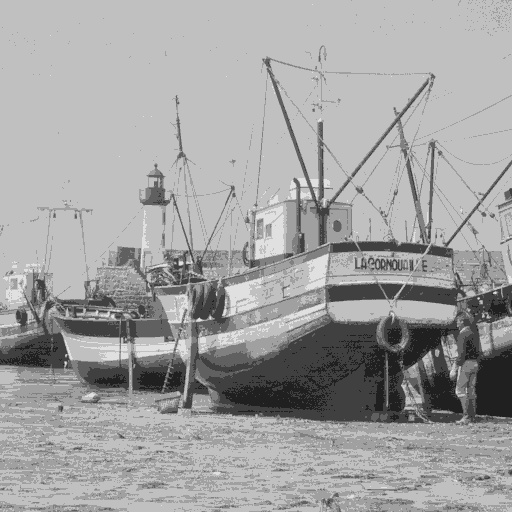
\includegraphics[scale=0.25]{../ImageRes/ImagedecodeeMICDAQ32.jpg} 
\caption{Images décodées en MICDA avec un pas de 2,8 et 32 }
\end{center}
\end{figure}

\begin{figure}[H]
\begin{center}
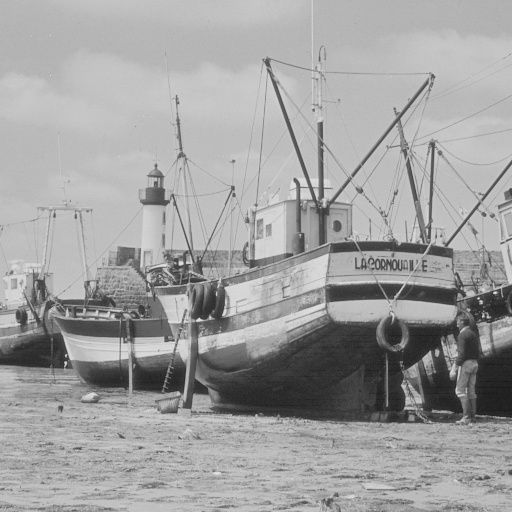
\includegraphics[scale=0.25]{../ImageRes/ImagedecodeeCompetitifQ2.jpg} 
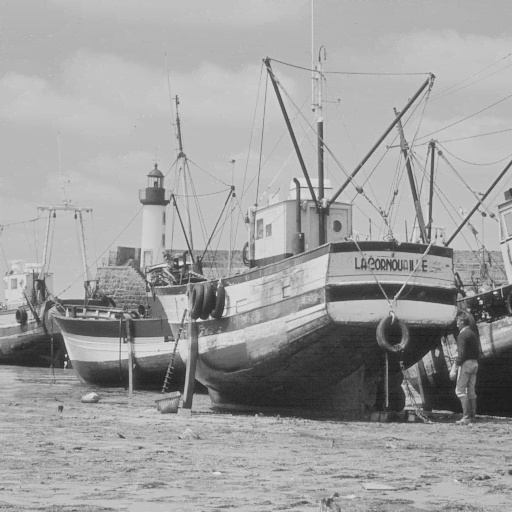
\includegraphics[scale=0.25]{../ImageRes/ImagedecodeeCompetitifQ8.jpg} 
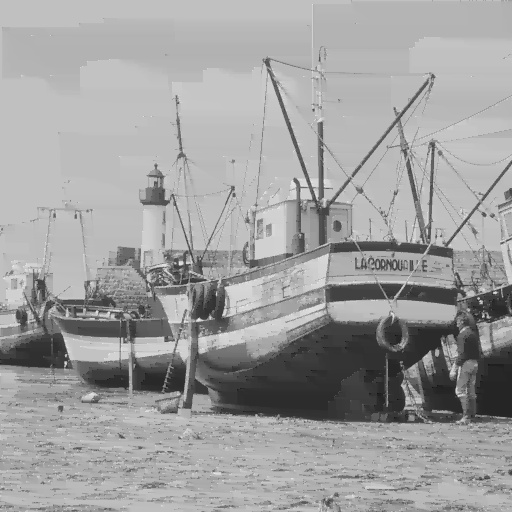
\includegraphics[scale=0.25]{../ImageRes/ImagedecodeeCompetitifQ32.jpg} 
\caption{Images décodées en compétitif avec un pas de 2,8 et 32 }
\end{center}
\end{figure}

Malgré tout, on peut observer que le compétitif résiste un peu mieux à la quantification et c'est notamment assez visible sur le graphique ci-dessous représentant le PSNR en fonction du pas de quantification. On voit que le compétitif est clairement au dessus des autres prédicteurs.

\begin{figure}[H]
\begin{center}
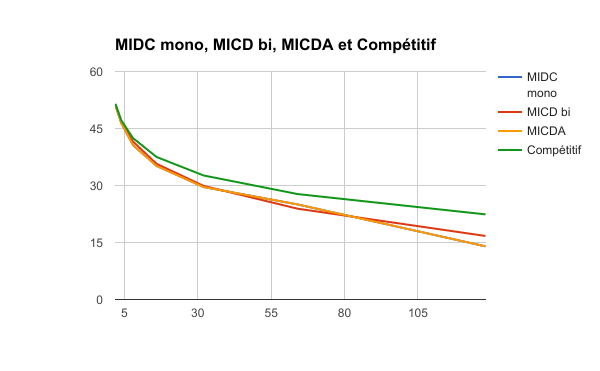
\includegraphics[scale=0.8]{../ImageRes/PSNR.png} 
\caption{PSNR en fonction du pas de quantification}
\end{center}
\end{figure}

\section{Conclusion}

Ce TP nous a permis de voir l’efficacité du schéma en boucle fermée et l'influence de la quantification sur cette structure. Nous avons aussi pu voir l'influence des différents prédicteurs sur l'image.


\begin{comment}

%Commande pour le sommaire

\renewcommand{\contentsname}{\large Sommaire} % Change le nom en sommaire
\setcounter{tocdepth}{2} % Défini la profondeur d'une table des matières
\tableofcontents
\newpage

\end{comment}

\newpage


%Commande pour le sommaire des figures

\renewcommand*\listfigurename{\large Liste des figures}
\listoffigures
\newpage


\end{document}
